%!TEX root = ../dissertation.tex
\chapter{Introduction}
\label{chap:introduction}
Computer simulation has opened up new research directions in many engineering and physical sciences. The increased reliance of engineers and scientists on computer modeling and simulation stems primarily from the relatively high cost of conducting experimental studies. Harnessing the power of today's computers to carry out billions of operations per second can translate in some cases in replacing large amounts of experimental work with effective computer simulation. In terms of continuum mechanics, current numerical methods can simulate problems with millions of degrees of freedom. Similarly, simulating the dynamics of many discrete systems with a relatively large number of degrees of freedom is possible. However, computer simulation of (i) multidisciplinary problems featuring the coupling of discrete systems and continua, and (ii) large scale discrete systems encountered in granular media continue to pose many and interesting challenges.

\section{Problem Statement}
Problems involving the interaction of multiple physical phenomena are prevalent in many engineering applications, ranging from biomechanics to geomechanics. Modeling and simulation of soft tissues or cardiovascular flows are prime examples of multi-physics problems in biomechanics. Many environmental applications concerning renewable energy devices, offshore wind turbines, etc., require modeling the dynamics of fluids, solids, and their interaction. Lastly, a multi-physics modeling and simulation capability is required in geomechanics problems encountered in partially saturated soil or landslides.   

From the computational perspective, simulation of discrete systems poses a higher computational burden comparing to continuum modeling. For instance, discrete modeling of soil and granular media leads to extremely large problems due to the small particle size and/or the large number of particles in many real-world problems. A continuum approximation of these systems could lead to more efficient solvers, yet the success of the homogenization process is dictated by the predictive attribute of suitably chosen constitutive laws. The interest in this Ph.D. thesis is in modeling the dynamics of both discrete and continuum systems as well as their coupling, and, when possible, to use the continuum approach to approximate discrete systems.

The problems of interest in this work span multiple disciplines across continuum and discrete systems as shown in Fig.~\ref{fig:Overview}. These problems include dynamics of (i) fluids, (ii) rigid and flexible multi-body systems, and (iii) fluid-solid interaction problems where dynamics of a continuum is coupled with discrete flexible or rigid multi-body systems. Owing to their multi-physics nature, these three thrusts cover a wide range of real-world applications that span multiple disciplines and industries. 
\begin{figure}[H]
	\begin{center}
		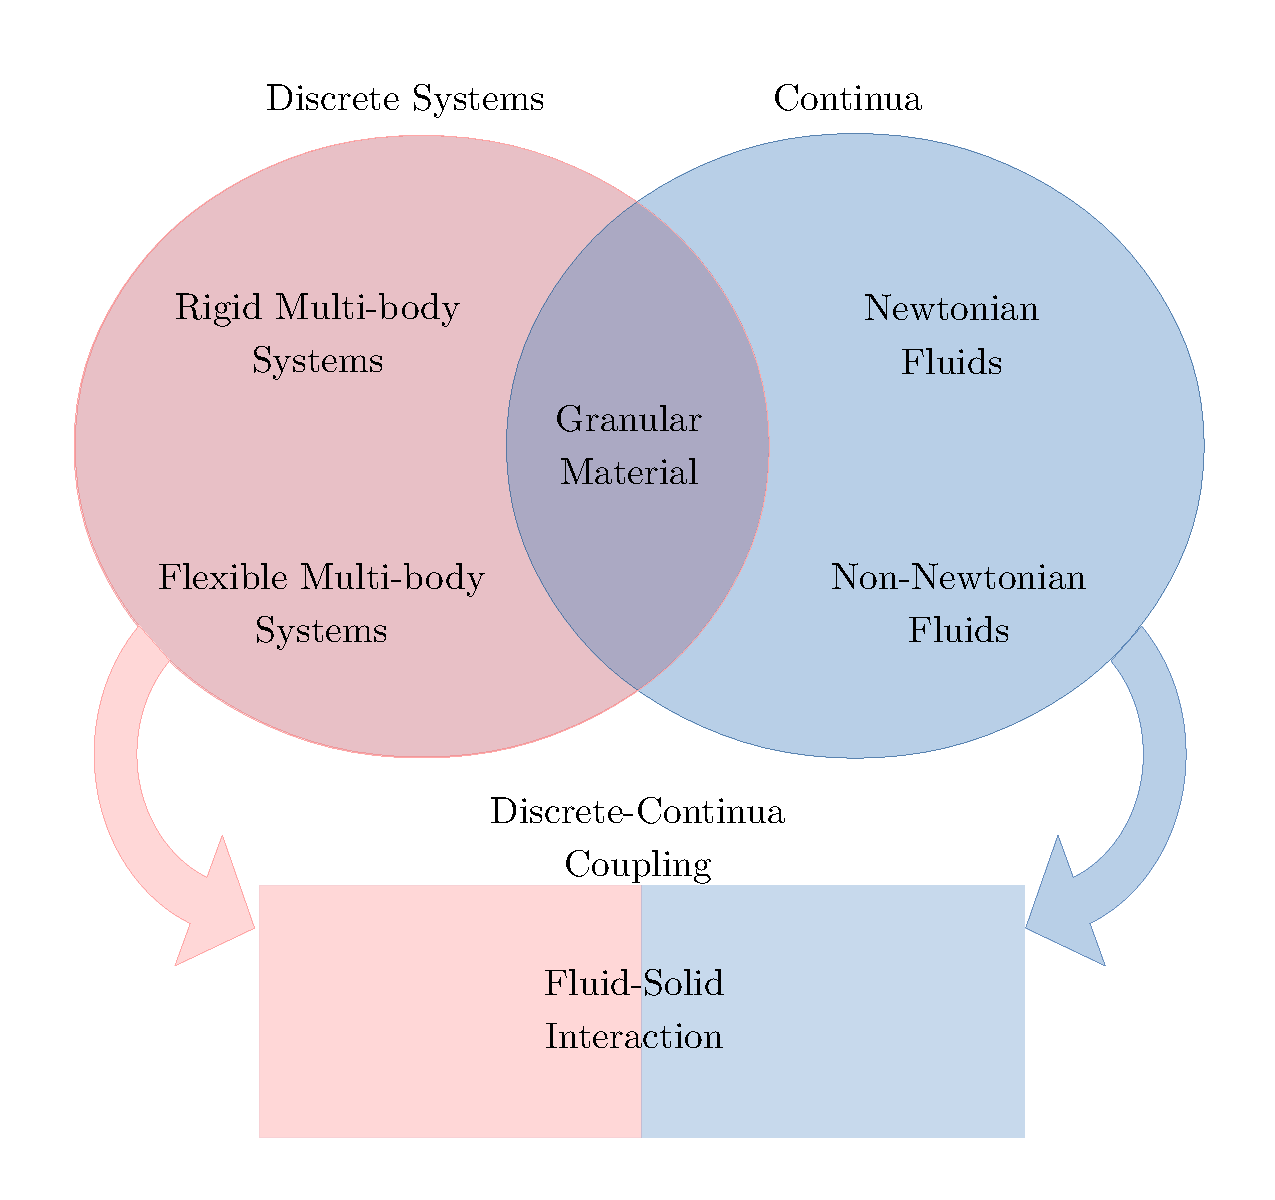
\includegraphics[width=.75\linewidth]{images/Overview.pdf}
	\end{center}
	\caption{Schematic overview of the problems of interest in the present thesis.}
	\label{fig:Overview}
\end{figure}


\section{Thesis Overview}
This manuscript is organized as follows: Chapter \ref{chap:background} will provide a brief overview of the existing work and literature on computational fluid dynamics, multi-body dynamics, and fluid-solid interaction. Chapters \ref{chap:discrete_Model} and \ref{chap:continua_Model} will discuss the modeling aspects and the numerical methods for solving the governing equations of discrete and continuous systems, respectively. Details about the software implementation of the  framework are presented in Chapter \ref{chap:implementation}, with numerical experiments and validation discussed in Chapter \ref{chap:experiments}. Chapter \ref{chap:demonstration} presents several applications and demonstrates the capabilities of the developed computational framework. Conclusions and directions of future work are discussed in Chapter \ref{chap:conclusions}.




\section{Summary of Contributions}
\label{sec:contributions}
The author's work has led to the following archival publications: \cite{miladSPHcomparison2019,lagrangianVSeulerian2019,miladHalfImplicit2018,rakhsha2019simulation,hammadConstrFluid2018,weiWenxiaoDanMultiresolution2017,miladASME2017}. The specific contributions of the author are summarized as follows:
\begin{compactitem} 
	\item Investigated the use of SPH for the Navier-Stokes equations
	\begin{compactitem} 
		\item Investigated four different SPH methods (WCSPH, ISPH, KCSPH, and IISPH) and  their solution attributes
		\item Performed a comparison between Implicit SPH (ISPH), Weakly Compressible SPH (WCSPH), and Kinematically Constrained SPH (KCSPH)
		\item Compared and contrasted the solution attributes of SPH as a Lagrangian method against continuous finite element method for free-surface and fluid-solid interaction problems 
		\item Implemented and improved the Implicit Incompressible SPH \cite{ihmsen2014implicit} method by solving the discretized Poisson pressure equation via advanced linear solvers
		\item Implemented and validated a projection-based implicit, both velocity and pressure, solver that can handle a wide range of fluid flows ranging from highly viscous flows to flows with moderately large Reynolds numbers in the laminar regime
		\item Investigated the use of consistent SPH discretization for internal flow problems
		\item Implemented the Herschel-Bulkley fluid model for modeling and simulation of non-Newtonian fluids
		\item Investigated the use of ISPH method for modeling and simulation of granular dynamics as a non-Newtonian fluid 
	\end{compactitem}
	

	\item Investigated the solution quality in frictional-contact problems and demonstrated insights gained in the context of a biomechanics application 
		\begin{compactitem} 
		\item  Investigated the use of the Tikhonov regularization method for imparting uniqueness to the distribution of frictional contact forces in granular dynamics problems solved via a differential variational inequality approach
		\item Simulated the tibiofemoral cartilage contact during walking for the prediction of collagen fiber orientation
	\end{compactitem}

	\item Developed a partitioned fluid-solid interaction framework
	\begin{compactitem} 
		\item  Coupled the fluid solver to a multi-body engine capable of simulating rigid and flexible bodies  interacting through frictional contact
		\item  Validated the fluid-structure coupling via benchmark experiments featuring flexible and rigid elements
	\end{compactitem}
	
	
	\item Leveraged hybrid CPU/GPU parallelization to improve the performance of the FSI framework 
	\begin{compactitem} 
		\item Implemented SPH on GPU cards using CUDA  to leverage high memory bandwidth
		\item Implemented Krylov linear solvers such as GMRES and BiCGStab on GPU to improve the efficiency of the underlying linear solvers
		\item Leveraged OpenMP for parallelism of the flexible multi-body dynamics solver on the CPU
		\item Improved the efficiency of the low-level matrix operation on the host code via AVX vectorization intrinsics
	\end{compactitem}
\end{compactitem} 